\title{Manual uso servidor GAIA}
\author{}
\documentclass[12pt]{article}
\usepackage{graphicx}
\graphicspath{ {./img/} }
\begin{document}
\maketitle
\tableofcontents
\section{Acceso al servidor}
Para acceder al servidor hay varias opciones. No hay una opci\'on mejor o peor, la elecci\'on de una de ellas depende de las necesidades.
\subsection{Secure Shell (SSH)}
SSH es un protocolo el cual sirve para acceder de forma remota a un servidor.
\subsubsection{Linux}
En las distribuciones linux, SSH ya viene instalado. Para acceder al servidor:
\begin{enumerate}
    \item Presione CTRL + ALT + t para abrir una terminal.
    \item En la terminal escriba el siguiente comando:
          \begin{verbatim}
my_username@host:$ ssh username@host_ip_address
\end{verbatim}
          donde \textbf{username} es el nombre de usuario del servidor al cual se desea ingresar; \textbf{host\_ip\_address} es la ip o el dominio de dicho servidor.
    \item Escriba la contrase\~na del usuario del servidor y presione Enter.
    \item Cuando se conecta a un servidor por primera vez, le preguntar\'a si desea continuar con la conexi\'on. Simplemente escriba si y pulse Enter. Este mensaje
          s\'olo aparece esta vez, ya que el servidor remoto no est\'a identificado en su m\'aquina local.
    \item Si lleg\'o hasta ac\'a, ya se encuentra conectado al servidor remoto. Puede escribir cualquier comando en la sesi\'on de terminal que
          tiene abierta y este ser\'a ejecutado en el servidor remoto.
\end{enumerate}
\subsubsection{Windows}
Los usuarios de Windows pueden usar PuTTY el cual es un cliente de SSH. A continuaci\'on los pasos para configurar PuTTY:
\begin{enumerate}
    \item Descargar el ejecutable desde https://www.putty.org/
    \item Una vez PuTTY es ejecutado se ver\'a como la Figura \ref{putty1}. En el campo \textbf{Host Name} se debe introducir el nombre o direcci\'on IP de
          la m\'aquina a la cual se va a aacceder. En el campo \textbf{Port} se debe introducir el puerto bajo el cual el servidor SSH esta corriendo. Lo usual es que el puerto sea el \textbf{22}.
    \item Despu\'es de llenar los campos, dar click en Open
    \item Si es la primera vez que se conecta al servidor desde su m\'aquina entonces el pedir\'a una confirmaci\'on. Aceptar la conexi\'on dando click en Yes.
    \item Una vez la conexi\'on SSH esta abierta aparecer\'a una terminal en la cual se debe digitar el usuario del servidor al que se quiere acceder.
    \item Ahora digitar la contrase\~na de dicho usuario.
    \item Ya se encuentra conectado al servidor v\'ia SSH y tiene una sesi\'on de terminal abierta, todo lo que digite en esta, ser\'a ejecutado en el servidor remoto.
\end{enumerate}
\begin{figure}[]
    \centering
    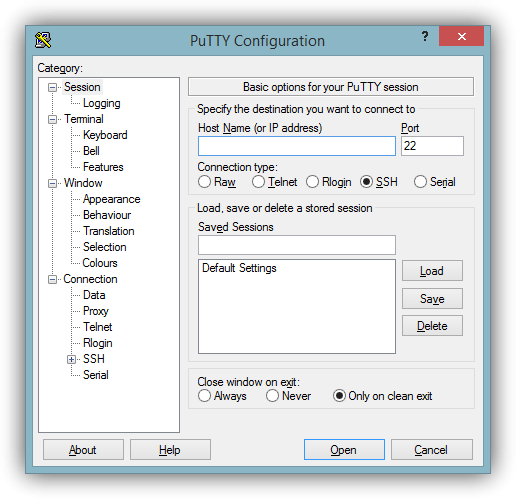
\includegraphics{putty-tutorial-foto-1.png}
    \caption{Pantalla principal de PuTTY}
    \label{putty1}
\end{figure}
\end{document}